\documentclass[11pt,a4paper]{article}
\usepackage[margin=2.2cm]{geometry}
\usepackage{amsmath}
\usepackage{graphicx}
\usepackage{float}
\usepackage{listings}

\lstset{basicstyle=\ttfamily\footnotesize, frame=single, numbers=left,
        numberstyle=\tiny, breaklines=true, columns=fullflexible, showstringspaces=false,
        literate={ı}{{\i}}1 {ş}{{\c{s}}}1 {ğ}{{\u{g}}}1 {ü}{{\"u}}1 {ö}{{\"o}}1 {ç}{{\c{c}}}1
                 {İ}{{\.I}}1 {Ş}{{\c{S}}}1 {Ğ}{{\u{G}}}1 {Ü}{{\"U}}1 {Ö}{{\"O}}1 {Ç}{{\c{C}}}1
                 {·}{{$\cdot$}}1}


\title{DEP521E -- HW3 Parts A and B\\Newton-Raphson Iteration with Newmark-$\beta$}
\author{Mesut ADALI - 801262107}
\date{16.11.2026}


\begin{document}
\maketitle

\section{Input Parameters}
\begin{table}[H]
\centering
\begin{tabular}{llrl}
\hline
Parameter & Symbol & Value & Units \\
\hline
Mass                & $m$   & 1000 & kg \\
Damping ratio       & $\xi$ & 2    & \% \\
Initial period      & $T$   & 1    & s \\
Primary stiffness   & $k_p = m(2\pi/T)^2$ & 39478.4 & N/m \\
Yield displacement  & $d_y$ & 7.5  & cm \\
Yield force         & $f_y = k_p d_y$ & 2960.9 & N \\
Secondary stiffness & $k_s = 0.1k_p$  & 3947.8 & N/m \\
\hline
\end{tabular}
\caption{SDOF system parameters.}
\end{table}


\section{Part A.1 -- Original Newton-Raphson}
\subsection{Method}
The Newmark average acceleration method (beta = 1/4, gama = 1/2) was employed. Since the spring exhibits nonlinear behavior, the total formulation was used.


\subsection{Command Line Output}
\begin{lstlisting}
iteration time: 0.026777799997944385
Yielding steps: 194
\end{lstlisting}

\subsection{Results}
Initial yielding occurs at approximately t=6.35 s. The maximum displacement is 21.46 cm, while the residual displacement is approximately 5.7 cm.
Two iterations are required only at time steps where the response transitions from the elastic range to the yielding threshold. Since the bilinear model is linear within each branch, the second iteration provides the exact solution.
\begin{figure}[H]
\centering
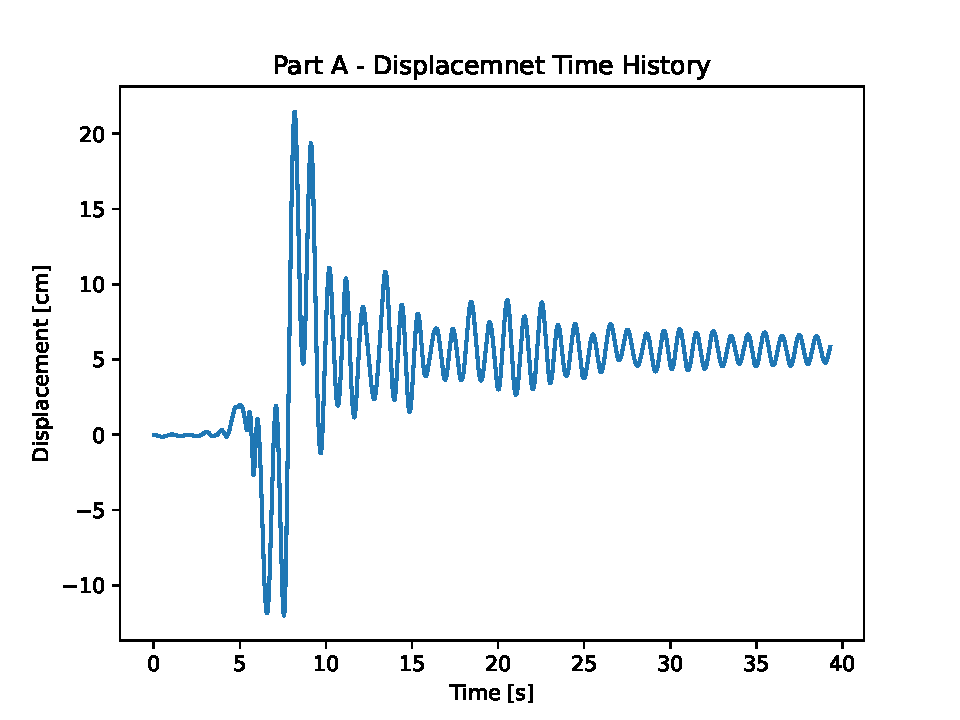
\includegraphics[width=0.49\textwidth, page=1]{PartA_results.pdf}
\includegraphics[width=0.49\textwidth, page=2]{PartA_results.pdf}
\caption{Displacement time history (left) and spring force time history (right).}
\end{figure}

\begin{figure}[H]
\centering
\includegraphics[width=0.6\textwidth, page=3]{PartA_results.pdf}
\caption{Displacement -- spring force hysteresis.}
\end{figure}

\begin{figure}[H]
\centering
\includegraphics[width=0.49\textwidth, page=4]{PartA_results.pdf}
\includegraphics[width=0.49\textwidth, page=5]{PartA_results.pdf}
\caption{Relative acceleration (left) and absolute acceleration (right) time histories.}
\end{figure}



\section{Part A.2 -- Modified Newton-Raphson}
\subsection{Method}
The only difference is that K is calculated once at the beginning of each time step using kT(state[i]) and remains constant throughout the iterations.
\subsection{Command Line Output}
\begin{lstlisting}
iteration time: 0.026309200009563938
Yielding steps: 194
\end{lstlisting}

\subsection{Results}
\begin{figure}[H]
\centering
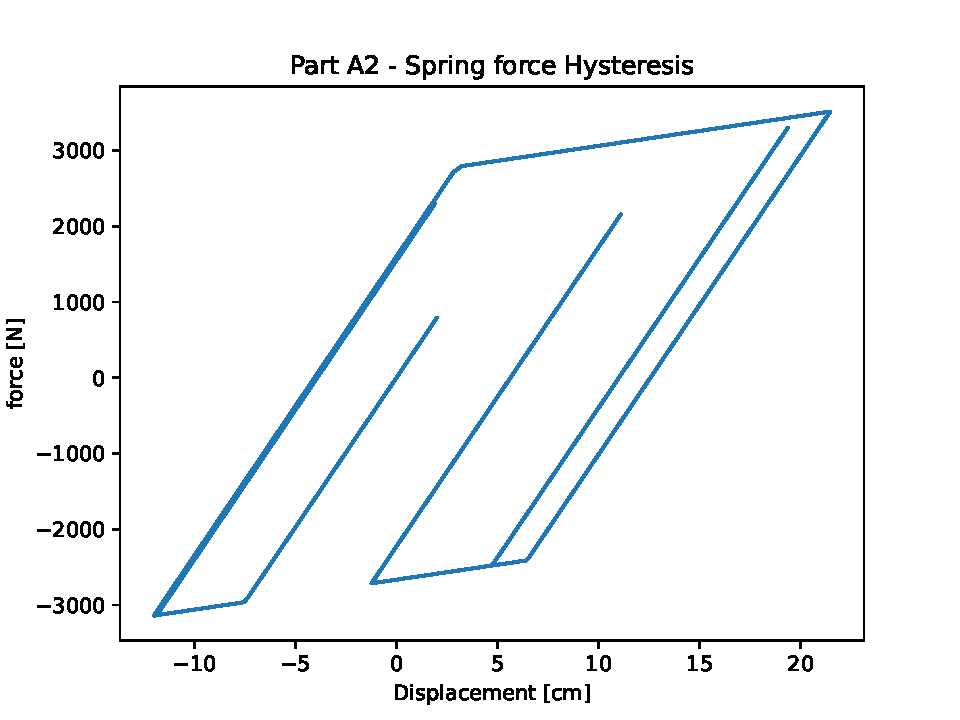
\includegraphics[width=0.6\textwidth]{PartA2_results.pdf}
\caption{Displacement -- spring force hysteresis, modified Newton-Raphson.}
\end{figure}



\section{Part B -- Comparison with the Linear System}


\begin{table}[H]
\centering
\begin{tabular}{lrr}
\hline
Quantity & Nonlinear & Linear \\
\hline
Max. displacement [cm]                  & 21.46 & 23.17 \\
Max. velocity [m/s]                     & 0.841 & 1.415 \\
Max. absolute acceleration [m/s$^2$]    & 3.545 & 9.156 \\
Max. spring force [N]                   & 3512  & 9149  \\
\hline
\end{tabular}
\caption{Maximum responses of the nonlinear and linear systems.}
\end{table}

\begin{figure}[H]
\centering
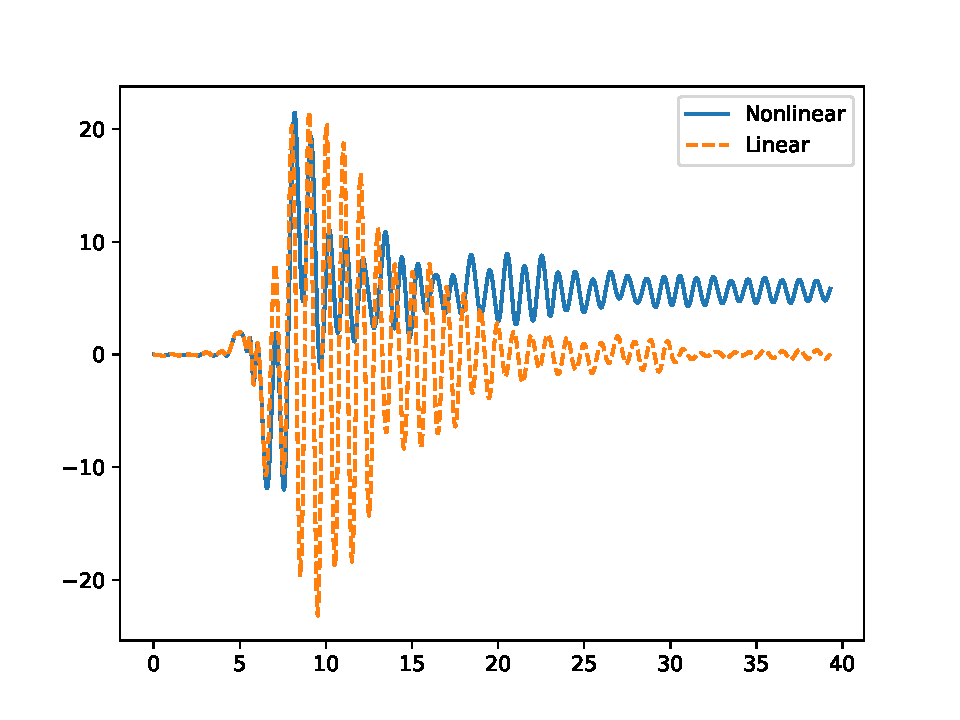
\includegraphics[width=0.8\textwidth]{PartB_results.pdf}
\caption{Displacement time history of the nonlinear and linear systems.}
\end{figure}



\appendix
\section{Python Code -- Part A.1 and Part B}
\lstinputlisting[language=Python]{NR.py}

\section{Python Code -- Part A.2}
\lstinputlisting[language=Python]{NR_modified.py}

\end{document}
